\documentclass[ignorenonframetext,]{beamer}
\setbeamertemplate{caption}[numbered]
\setbeamertemplate{caption label separator}{: }
\setbeamercolor{caption name}{fg=normal text.fg}
\beamertemplatenavigationsymbolsempty
\usepackage{lmodern}
\usepackage{amssymb,amsmath}
\usepackage{ifxetex,ifluatex}
\usepackage{fixltx2e} % provides \textsubscript
\ifnum 0\ifxetex 1\fi\ifluatex 1\fi=0 % if pdftex
  \usepackage[T1]{fontenc}
  \usepackage[utf8]{inputenc}
\else % if luatex or xelatex
  \ifxetex
    \usepackage{mathspec}
  \else
    \usepackage{fontspec}
  \fi
  \defaultfontfeatures{Ligatures=TeX,Scale=MatchLowercase}
\fi
\usetheme[]{Copenhagen}
\usecolortheme{dolphin}
\usefonttheme{structurebold}
% use upquote if available, for straight quotes in verbatim environments
\IfFileExists{upquote.sty}{\usepackage{upquote}}{}
% use microtype if available
\IfFileExists{microtype.sty}{%
\usepackage{microtype}
\UseMicrotypeSet[protrusion]{basicmath} % disable protrusion for tt fonts
}{}
\newif\ifbibliography
\hypersetup{
            pdftitle={1- Introduction to the R language},
            pdfauthor={Alex Sanchez, Miriam Mota, Ricardo Gonzalo and Mireia Ferrer},
            pdfborder={0 0 0},
            breaklinks=true}
\urlstyle{same}  % don't use monospace font for urls

% Prevent slide breaks in the middle of a paragraph:
\widowpenalties 1 10000
\raggedbottom

\AtBeginPart{
  \let\insertpartnumber\relax
  \let\partname\relax
  \frame{\partpage}
}
\AtBeginSection{
  \ifbibliography
  \else
    \let\insertsectionnumber\relax
    \let\sectionname\relax
    \frame{\sectionpage}
  \fi
}
\AtBeginSubsection{
  \let\insertsubsectionnumber\relax
  \let\subsectionname\relax
  \frame{\subsectionpage}
}

\setlength{\parindent}{0pt}
\setlength{\parskip}{6pt plus 2pt minus 1pt}
\setlength{\emergencystretch}{3em}  % prevent overfull lines
\providecommand{\tightlist}{%
  \setlength{\itemsep}{0pt}\setlength{\parskip}{0pt}}
\setcounter{secnumdepth}{0}

\title{1- Introduction to the R language}
\author{Alex Sanchez, Miriam Mota, Ricardo Gonzalo and Mireia Ferrer}
\date{Statistics and Bioinformatics Unit. Vall d'Hebron Institut de Recerca}

\begin{document}
\frame{\titlepage}

\begin{frame}{Readme}

\begin{itemize}
\item
  License: Creative Commons Attribution-NonCommercial-ShareAlike 4.0
  International License
  \url{http://creativecommons.org/licenses/by-nc-sa/4.0/}
\item
  You are free to:

  \begin{itemize}
  \tightlist
  \item
    \textbf{Share} : copy and redistribute the material
  \item
    \textbf{Adapt} : rebuild and transform the material
  \end{itemize}
\item
  Under the following conditions:

  \begin{itemize}
  \tightlist
  \item
    \textbf{Attribution} : You must give appropriate credit, provide a
    link to the license, and indicate if changes were made.
  \item
    \textbf{NonCommercial} : You may not use this work for commercial
    purposes.
  \item
    \textbf{Share Alike} : If you remix, transform, or build upon this
    work, you must distribute your contributions under the same license
    to this one.
  \end{itemize}
\end{itemize}

\end{frame}

\section{Introduction to R}\label{introduction-to-r}

\begin{frame}{Outline}

\begin{itemize}
\tightlist
\item
  A first contact with R \& Rstudio.

  \begin{itemize}
  \tightlist
  \item
    How does one work with R
  \end{itemize}
\item
  A primer of data import

  \begin{itemize}
  \tightlist
  \item
    Reading data into R
  \end{itemize}
\item
  A primer of communication

  \begin{itemize}
  \tightlist
  \item
    R Notebooks and RMarkdown
  \end{itemize}
\end{itemize}

\end{frame}

\section{\texorpdfstring{A first contact with R, Rstudio and the
\texttt{tidyverse}}{A first contact with R, Rstudio and the tidyverse}}\label{a-first-contact-with-r-rstudio-and-the-tidyverse}

\begin{frame}{\href{https://www.r-project.org/about.html}{What is R?}}

\begin{itemize}
\item
  R is a \emph{language and environment} for statistical computing and
  graphics.
\item
  R provides a wide variety of statistical and graphical techniques, and
  is highly extensible.
\item
  It compiles and runs on a wide variety of UNIX platforms and similar
  systems Windows and MacOS.
\end{itemize}

\end{frame}

\begin{frame}{R PRO's (why you are here!)}

\begin{itemize}
\tightlist
\item
  The system is

  \begin{itemize}
  \tightlist
  \item
    free (as in \emph{free beer})
  \item
    It's platform independent
  \item
    It is constantly improving (2 new versions/year)
  \end{itemize}
\item
  It is a statistical tool

  \begin{itemize}
  \tightlist
  \item
    Implements almost every statistical method that exists
  \item
    Great graphics (Examples)
  \item
    Simple reporting tools
  \item
    Also state-of-the-art in Bioinformatics through the
    \href{http://bioconductor.org}{Bioconductor Project}.
  \end{itemize}
\item
  Programming language

  \begin{itemize}
  \tightlist
  \item
    Easy to automate repetitive tasks (Example\_1.1)
  \item
    Possibility to create user friendly web interfaces with a moderate
    effort. (Examples)
  \end{itemize}
\end{itemize}

\end{frame}

\begin{frame}{R CON's}

\begin{itemize}
\item
  R is mainly used issuing commands from a console

  \begin{itemize}
  \tightlist
  \item
    less user friendly that almost any other statistical tool you may
    know.
  \end{itemize}
\item
  Constantly having new versions may affect our projects
\item
  Not necessarily the best language nor suitable for every existing task
\end{itemize}

\end{frame}

\begin{frame}{How is R used}

\begin{itemize}
\item
  Traditionally R was used from an Operating System console
  (``Terminal'')
\item
  This is an intimidating approach for many users
\item
  A variety of options exist to decrease the learning curve.

  \begin{itemize}
  \tightlist
  \item
    Use a supportive development environment such as \textbf{Rstudio}
  \item
    Use an interface to Statistical tools, such as \textbf{Rcommander}
    or ::DeduceR** allowing to concetrate an Statistics, not in
    commands.
  \end{itemize}
\end{itemize}

\end{frame}

\begin{frame}{A raw R console in linux}

\begin{figure}
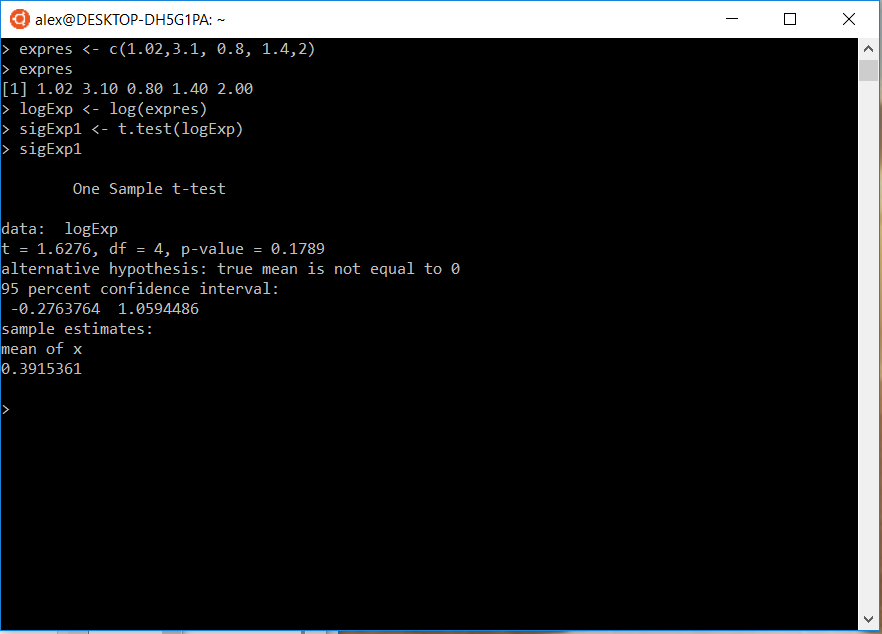
\includegraphics[width=0.85\linewidth]{images/RConsole.png}
\end{figure}

\end{frame}

\begin{frame}{An ``enhanced'' console: Rstudio}

\begin{figure}
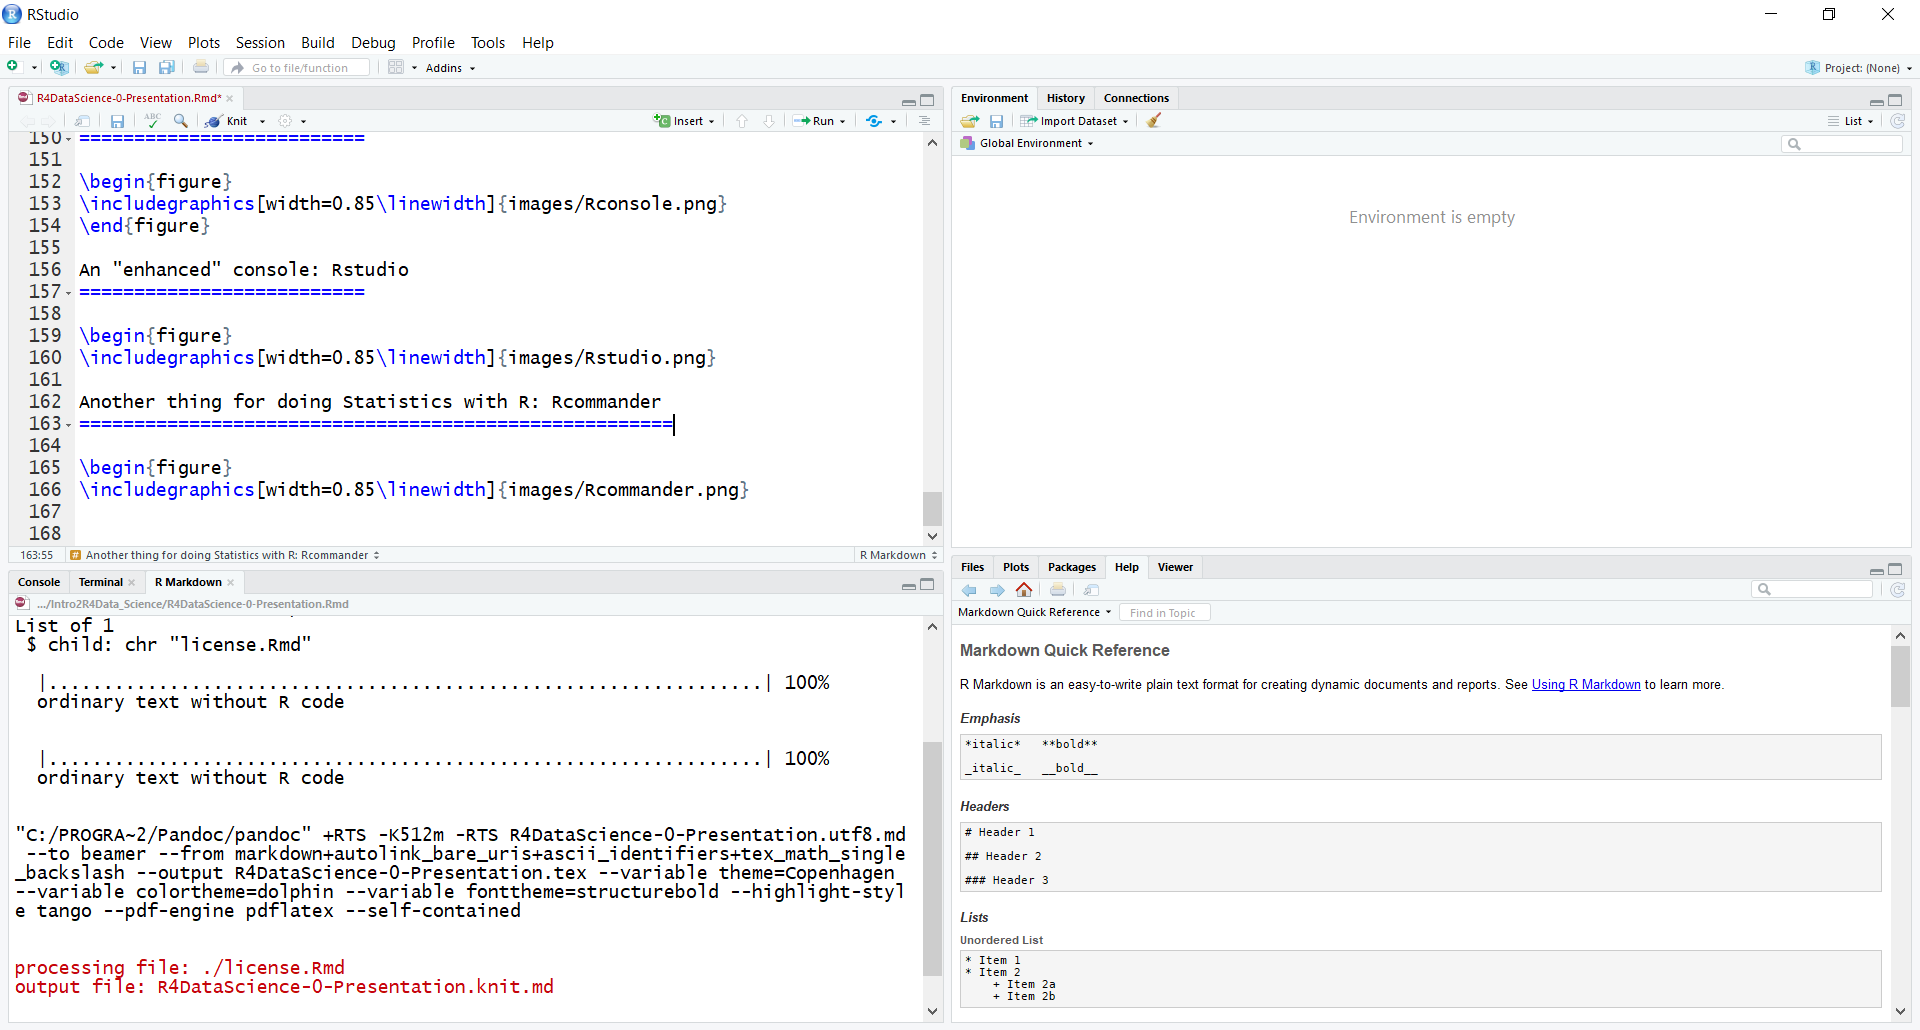
\includegraphics[width=0.85\linewidth]{images/RStudio.png}
\end{figure}

\end{frame}

\begin{frame}{Something that is not a console: Rcommander}

\begin{figure}
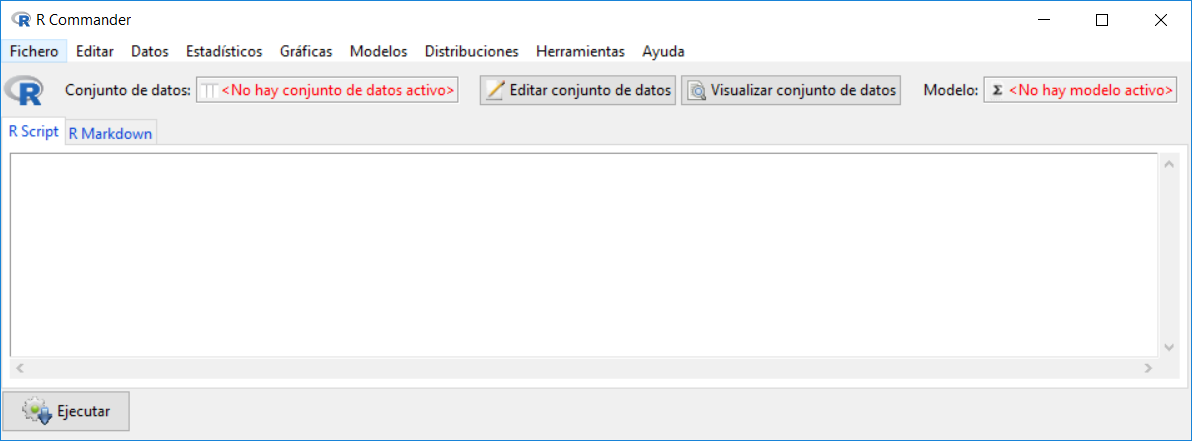
\includegraphics[width=0.85\linewidth]{images/RCommander.png}
\end{figure}

\end{frame}

\section{Using R}\label{using-r}

\begin{frame}{Commands, Objects and Functions}

Some explanations here

\end{frame}

\begin{frame}{Packages and datasets}

Some explanations here

\end{frame}

\begin{frame}{The \texttt{tidyverse}}

Some explanations here

\end{frame}

\begin{frame}{Some basic data types}

Some explanations here

\end{frame}

\section{Getting data into R}\label{getting-data-into-r}

\begin{frame}{Importing data with Rstudio}

Some explanations here

\end{frame}

\begin{frame}{Reading Excel files}

Some explanations here

\end{frame}

\begin{frame}{Reading text files}

Some explanations here

\end{frame}

\begin{frame}{Interlude: Summarizing data}

Some explanations here

\end{frame}

\section{Dynamic output with
Rmarkdown}\label{dynamic-output-with-rmarkdown}

\begin{frame}{Reproducible research with R notebooks}

Some explanations here

\end{frame}

\begin{frame}{Dynamic reports with Rmarkdown}

Some explanations here

\end{frame}

\end{document}
